\section{GUI}\label{sec:gui}

Interfejs graficzny składać się będzie z kilku części. Panel opcji w lewym dolnym rogu zawierać będzie przyciski do zapisu i odczytu symulacji, tworzenia nowych planet oraz wstrzymywania symulacji. W prawym dolnym rogu znajdą się dwa suwaki służące do kontroli prędkości symulacji oraz kamery. W głównej części ekranu znajdzie się najważniejsza część, czyli widok z kamery. Dodatkowo, po zaznaczeniu planety, pojawi się okienko z informacjami o niej - takimi jak położenie, prędkość czy masa. W tymże okienku można także wcisnąć przycisk usuwający planetę.

\begin{figure}[h]
	\centering
	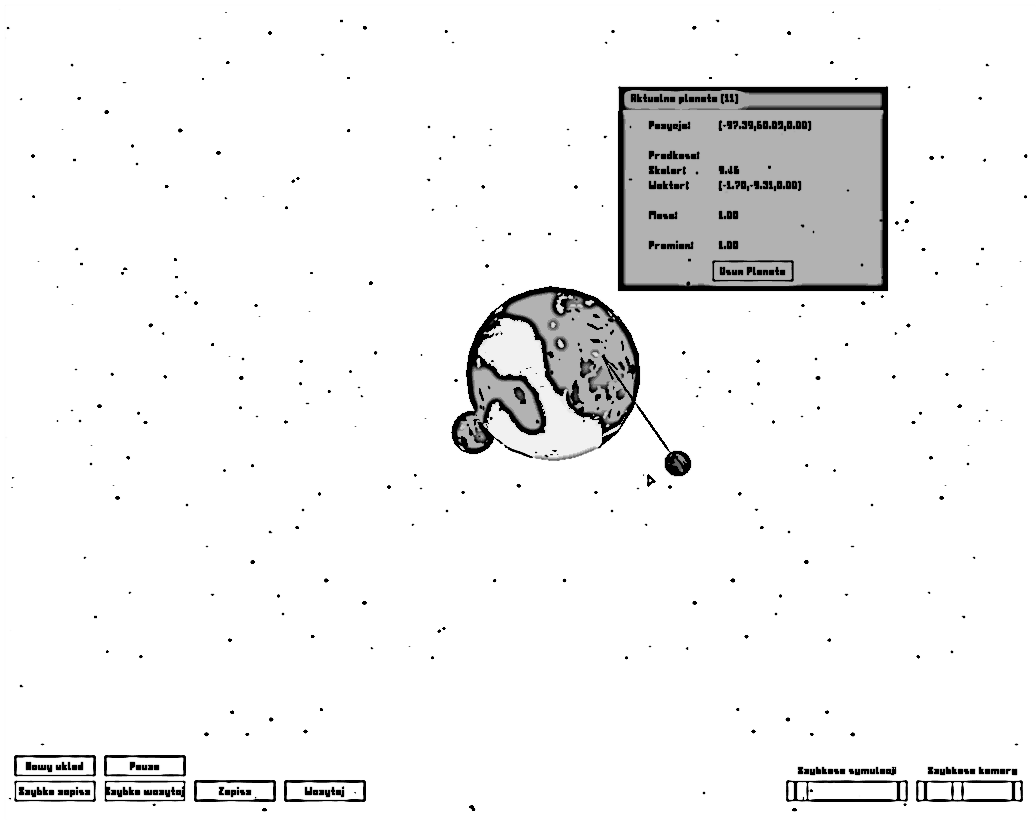
\includegraphics[width=1.0\textwidth]{gui.png}
	\caption{Prototyp interfejsu}
	\label{fig:gui}
\end{figure}

